\documentclass[14pt, a2paper, portrait]{tikzposter}
\usepackage[brazil]{babel}
\usepackage[utf8]{inputenc}
\usepackage[T1]{fontenc}
\usepackage{lipsum}
\usepackage{pdfpages} 
\newcommand{\bs}{\textbackslash}   
\newcommand{\cmd}[1]{{\bf \color{red}#1}}   
\tikzposterlatexaffectionproofon

\title{Um {\LaTeX} Sayajin}
\author{Guilherme Oliveira de Souza
\\\texttt{guilherme.ryders@gmail.com}}
\institute{Centro Universitário Senac}

 % Set colortheme
 % (default, anil, armin, edgar, emre, hanna, james, kai, lena, manuel,
 % martin, max, nicolas, pascal, peter, philipp, richard, roman, stefanie,
 % vinay)
\usecolortheme{nicolas}
\definecolor{framecolor}{named}{black}
\settitlebodystyle{rectangular}
\setblocktitlestyle{rounded}
\setblockbodystyle{shaded}

\begin{document}

\titleblock[left fig=logo.PNG, embedded]

\block[l]{Introdução}{
Este projeto foi feito em {\LaTeX} e é baseado em um desenho animado japonês chamado Dragon Ball, atualmente inpirado em sua temporada mais atual (Dragon Ball Super) criado por Akira Toriyama, sendo um desenho de grande sucesso que me veio à mente assim que foi dito como o projeto deveria ser feito. Mostrando a última evolução e demonstração de poder dos dois personagens principais do desenho animado: Goku e Vegeta em sua forma de Super Sayajin Blue.
}

\begin{columns}
% 1a coluna
\column{0.48}

\block[c]{Materiais e Métodos}{
Foram utilizados alguns programas de edição de imagem na imagem original, sendo eles: GIMP e Photoshop. O Photoshop foi usado para retirar o fundo da imagem original, deixá-lo transparente, e diminuir a opacidade da imagem para poder ficar mais visíveis as linhas criadas no projeto. O GIMP foi usado para conseguir as cores em RGB de cada parte da imagem para poder realizar a "pintura" da mesma.
Para compilar e editar o projeto em {\LaTeX}, foi utilizado o MikTex, TexStudio e o ShareLatex, tanto no Windows como Linux e Web (Sharelatex). Os pacotes utilizados foram (graphicx) para inserir a imagem, (tikz) para desenhar, e (color) para utilizar as cores em RGB no projeto. Antes de iniciar o desenho em si, adicionei a imagem original sem fundo e com a opacidade reduzida com o comando (includegraphics).
Imagem Referência:\\
    \begin{center}
      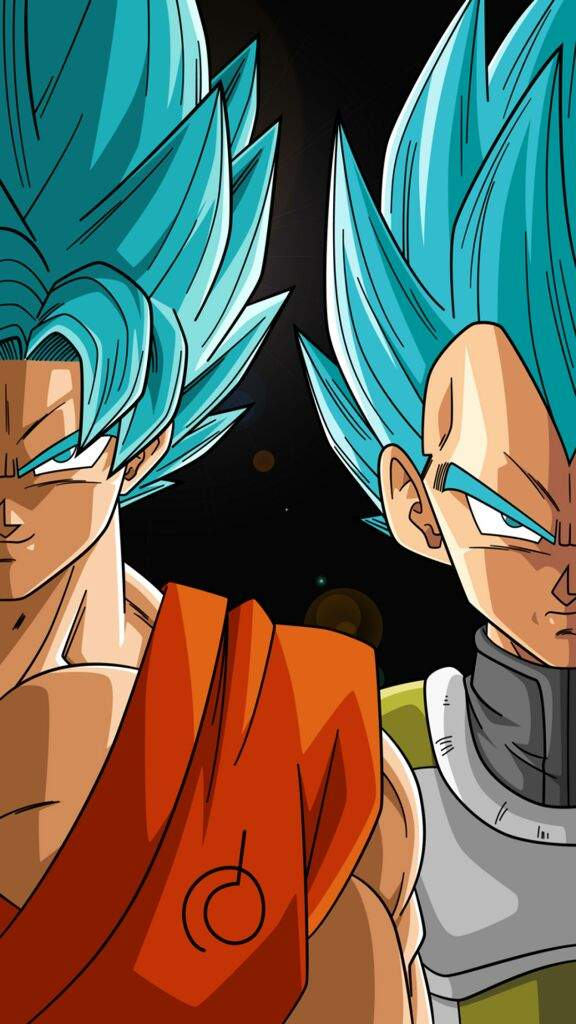
\includegraphics[width=7cm,height=12cm]{GVBOrig.jpg}  
    \end{center}
}

% 2a coluna
\column{0.52}

\block[c]{Resultado}{
    \begin{center}
        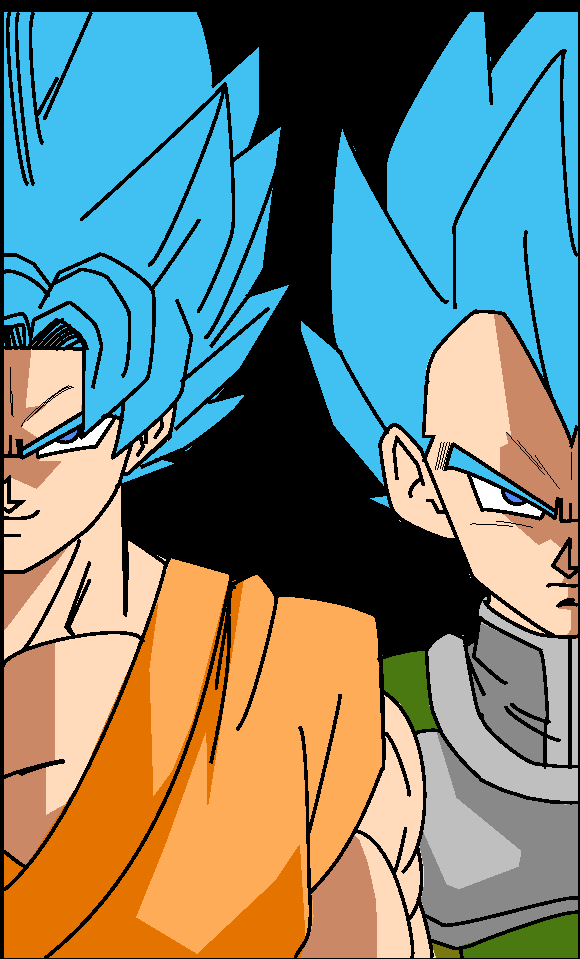
\includegraphics[width=9cm,height=15cm]{Goku_and_Vegeta_Blue(3).pdf}
    \end{center}
}

\block{Considerações Finais}{
Inicialmente não esperava que fosse possível utilizar uma linguagem para criar desenhos e imagens, o {\LaTeX} superou as minhas expectativas. O projeto resultou em novas interações na sala de aula e em troca de experiências entre os discentes e colegas de classe para que o projeto atingisse o resultado final desejado.
}

\end{columns}

\block[c,width=30cm]{Referências}{
\begingroup
   \renewcommand{\section}[2]{}
   \begin{thebibliography}{10}
	
	    \bibitem{Oetiker} OETIKER, Tobias et. al. {\sl Introdução ao {\LaTeXe}}, 2001.
	    \bibitem{Tantau} TANTAU, Till. {\sl The TikZ and PGF Packages}, http://www.texample.net/tikz/, 2014.
		\bibitem{Richter} RICHTER, Pascal et. al. {\sl The TikZposter class}, http://www.ctan.org/pkg/tikzposter/, 2014.

   \end{thebibliography}
\endgroup
}

\end{document}


